\section{Forward Problem: Proof 1F}
\label{sec:forward-problem-hodograph}
\subsection{Historical Hodograph Background}

\subsubsection{Newton, uniqueness, and asserted conics}

From the \emph{Principia} viewpoint (1687), Newton gives a geometric proposition-chain establishing both directions: conic with force at a focus $\Rightarrow$ inverse-square law, and inverse-square centripetal attraction $\Rightarrow$ conic orbits (ellipse/parabola/hyperbola by regime) \cite{newton1846mottewikisource,chandrasekhar1995principia}. What he does \emph{not} provide is a modern initial-value existence/uniqueness theorem for the forward problem; the argument is synthetic and limit-geometric (ultimate ratios), not an ODE well-posedness proof.

In parallel, early Continental analysts (late 17th to early 18th century) reduced the central-force problem by $u(\theta)=1/r$, yielding Binet's equation. For $F(r)=-\mu/r^2$:
\begin{equation}
  u''(\theta)+u=\frac{\mu}{h^2},
\end{equation}
with solution
\begin{equation}
  u(\theta)=\frac{\mu}{h^2}\Bigl(1+e\cos(\theta-\theta_0)\Bigr),
\end{equation}
i.e. a conic in polar form. However, deriving this form by itself is not a substitute for a uniqueness theorem: without an existence/uniqueness framework, one has not yet formalized exclusion of other possible local branches/continuations. Historical accounts of this transition to differential methods are discussed by Nauenberg (2003) \cite{nauenberg2003keplerarea}.

So the modern statement ``initial data determine a unique orbit'' is best read as a reconstruction of Newton's practice rather than a theorem he states in contemporary form. The same caution applies to early Continental differential reductions: the orbit equation gives candidate solution families, while later uniqueness theory is what formally secures single-orbit determinacy from initial data. Likewise, hodograph language is absent in the \emph{Principia} (1687) and appears later with Hamilton (1847). Rigorous local existence/uniqueness theorems for ODEs were developed much later (Cauchy in the 1820s; then Lipschitz/Picard--Lindel\"of in the late 19th century, roughly the 1870s--1890s), i.e. more than a century after 1687.

\subsubsection{Hamilton's circular hodograph for the inverse-square law}

Hamilton introduced the hodograph in 1847 as the curve traced by the tip of the velocity vector $\mathbf v(t)$ in velocity space, and showed that for motion under a central inverse-square force the hodograph is a circle \cite{hamilton1847hodograph}. Our proofs use this as a key starting point. Without offering new insights to this part, we simply explain the modern proof and refer to Feynman's work for a discrete version of the same argument \cite{goodstein1996feynman}.

Write the dynamics as
\[
  \ddot{\mathbf r}=-\frac{\mu}{r^2}\,\hat{\mathbf r},
  \qquad
  L:=r^2\dot\theta=\text{const}.
\]
Reparametrize by $\theta$:
\begin{equation}
  \frac{d\mathbf v}{d\theta}
  =
  \frac{d\mathbf v}{dt}\frac{dt}{d\theta}
  =
  \ddot{\mathbf r}\,\frac{r^2}{L}
  =
  -\frac{\mu}{L}\,\hat{\mathbf r}.
\label{eq:hodo-step1}
\end{equation}
Using the polar-frame identity
\[
  \frac{d\hat{\boldsymbol\theta}}{d\theta}=-\hat{\mathbf r},
\]
equation~\eqref{eq:hodo-step1} becomes
\begin{equation}
  \frac{d\mathbf v}{d\theta}
  =
  \frac{\mu}{L}\frac{d\hat{\boldsymbol\theta}}{d\theta}.
\label{eq:hodo-step2}
\end{equation}
Integrating once gives
\begin{equation}
  \frac{d}{d\theta}\!\left(\mathbf v-\frac{\mu}{L}\hat{\boldsymbol\theta}\right)=0
  \quad\Longrightarrow\quad
  \mathbf v=\mathbf C+\frac{\mu}{L}\hat{\boldsymbol\theta}.
\label{eq:hodo-step3}
\end{equation}
with constant vector $\mathbf C$.
Because $\|\hat{\boldsymbol\theta}\|=1$,
\[
  \|\mathbf v-\mathbf C\|=\frac{\mu}{L}.
\]
Hence the hodograph (the tip of $\mathbf v$ in velocity space) is a circle of radius $\mu/L$, centered at $\mathbf C$. Feynman provided a discrete argument without this vector derivatives which is essentially the same concept \cite{goodstein1996feynman}. If we change $d$ operator to $\Delta$ in the above argument, then it becomes
\begin{equation}
  \Delta\mathbf v = \frac{\mu}{L}\,\Delta\hat{\boldsymbol \theta}.
\label{eq:hodo-step1-discrete}
\end{equation}
This should already describes a constant curvature velocity-space curve, which is a circle of radius $\mu/L$, with its center to the force center since we also know both $\Delta\mathbf{v}$ and $\Delta\hat{\boldsymbol\theta}$ are in the radius direction. Feynman give a clear presentation on this descrte argument \cite{goodstein1996feynman}.

This fact is opposit to what we shows in previous sections, where we have established the conic sections together with constant areal speed (equivalently under central force) is sufficient condition for the hodograph to be a circle. It turns out that historically this circular-hodograph has become one central piece of evidence to help on both the inverse problem as well as the forward problem \cite{maxwell1877mattermotion,derbes2001reinventing,goodstein1996feynman,carinena2016newlook}. In later part of the section we will show how the forward problem can be solved nicely using two methods.

\subsubsection{Feynman's Lost Lecture, strengths, and later repairs}

Feynman's 1964 lecture re-popularized the hodograph method for teaching: first establishing a circular hodograph for inverse-square attraction, then reconstructing the conic orbit geometrically \cite{goodstein1996feynman}. Later work, including Derbes (2001), clarified missing details in tangent placement and invariants; in particular, angular momentum conservation (or the centripedal nature of the force) is the extra ingredient that fixes line placement and scale \cite{derbes2001reinventing}. More recent refinements, including van Haandel--Heckman (2009) and follow-up work by Cari\~nena--Ra\~nada--Santander (2016), may be read as using either (i) the directrix circle centered at the second focus, or (ii) an equivalent directrix-circle/hodograph picture centered at the force center, with a $\pm 90^\circ$ rotation between velocity and geometric proxy \cite{vanhaandelheckman2009teaching,carinena2016newlook}. CRS16 emphasizes that the force-center version gives a cleaner Feynman-style transformation.

In our constructions (\Cref{fig:hyperbola,fig:parabola-proof2}), the auxiliary circle has the same dual role. In particular, from the local identity used in \Cref{lem:product-identity},
\[
  FH\cdot FK' = b^2,
  \qquad
  F'\!A' = FK',
\]
so $\overrightarrow{F'\!A'}$ and $\overrightarrow{FK'}$ are colinear with opposite orientation and equal magnitude. Hence one can use the auxiliary-circle data with either center choice ($F$ or $F'$) as a hodograph proxy, corresponding to a $+90^\circ$ or $-90^\circ$ rotation. For the parabola, four equivalent rotated-hodograph constructions as shown in \cref{fig:parabola-proof2}; Derbes' choice is one of them (his $C_4$ circle). There are various different insights to it by viewing them each. The remaining step is the energy classification: $E<0$ gives an ellipse, $E=0$ the parabolic limit, and $E>0$ a hyperbola, or equivalently with the focus be inside/on/outside the hodograph circle, respectively.

\subsection{infinitesimal Hodograph Construction for the Forward Problem}

We take as given (from the historical discussion above) the hodograph-circle fact: for planar motion under a central inverse-square force, the hodograph of $\mathbf v(t)$ is a circle in velocity space.

Our goal is to recover the orbit form $r(\theta)$ (forward problem) by a finite-step argument aligned with Newton's impulse-triangle logic, minimizing reliance on continuous calculus.

In the next section, inspired by the geometric methods above, we give a forward-proof route based on explicit geometric construction. In the present section, however, we first take a slightly different approach: an infinitesimal hodograph analysis (Proof~1F).

\subsubsection{Instantaneous view of Hodograph as Proof 1F}

Assume planar motion under a centripetal acceleration toward $F$:
\begin{equation}
  a=\frac{\mu}{r^2},
  \qquad
  r=FA,
\end{equation}
and constant specific angular momentum
\begin{equation}
  L=r^2\dot\theta.
\end{equation}
Fix a small time step $\Delta t$, with consecutive points $B\to A$ on the orbit, $BR\perp FA$, and the translated $\Delta t$-scaled hodograph geometry in which
\begin{equation}
  OM=BR+OR'.
\end{equation}
Define
\begin{equation}
  u:=\frac{\mu}{L}.
\end{equation}

\begin{figure}[t]
  \centering
  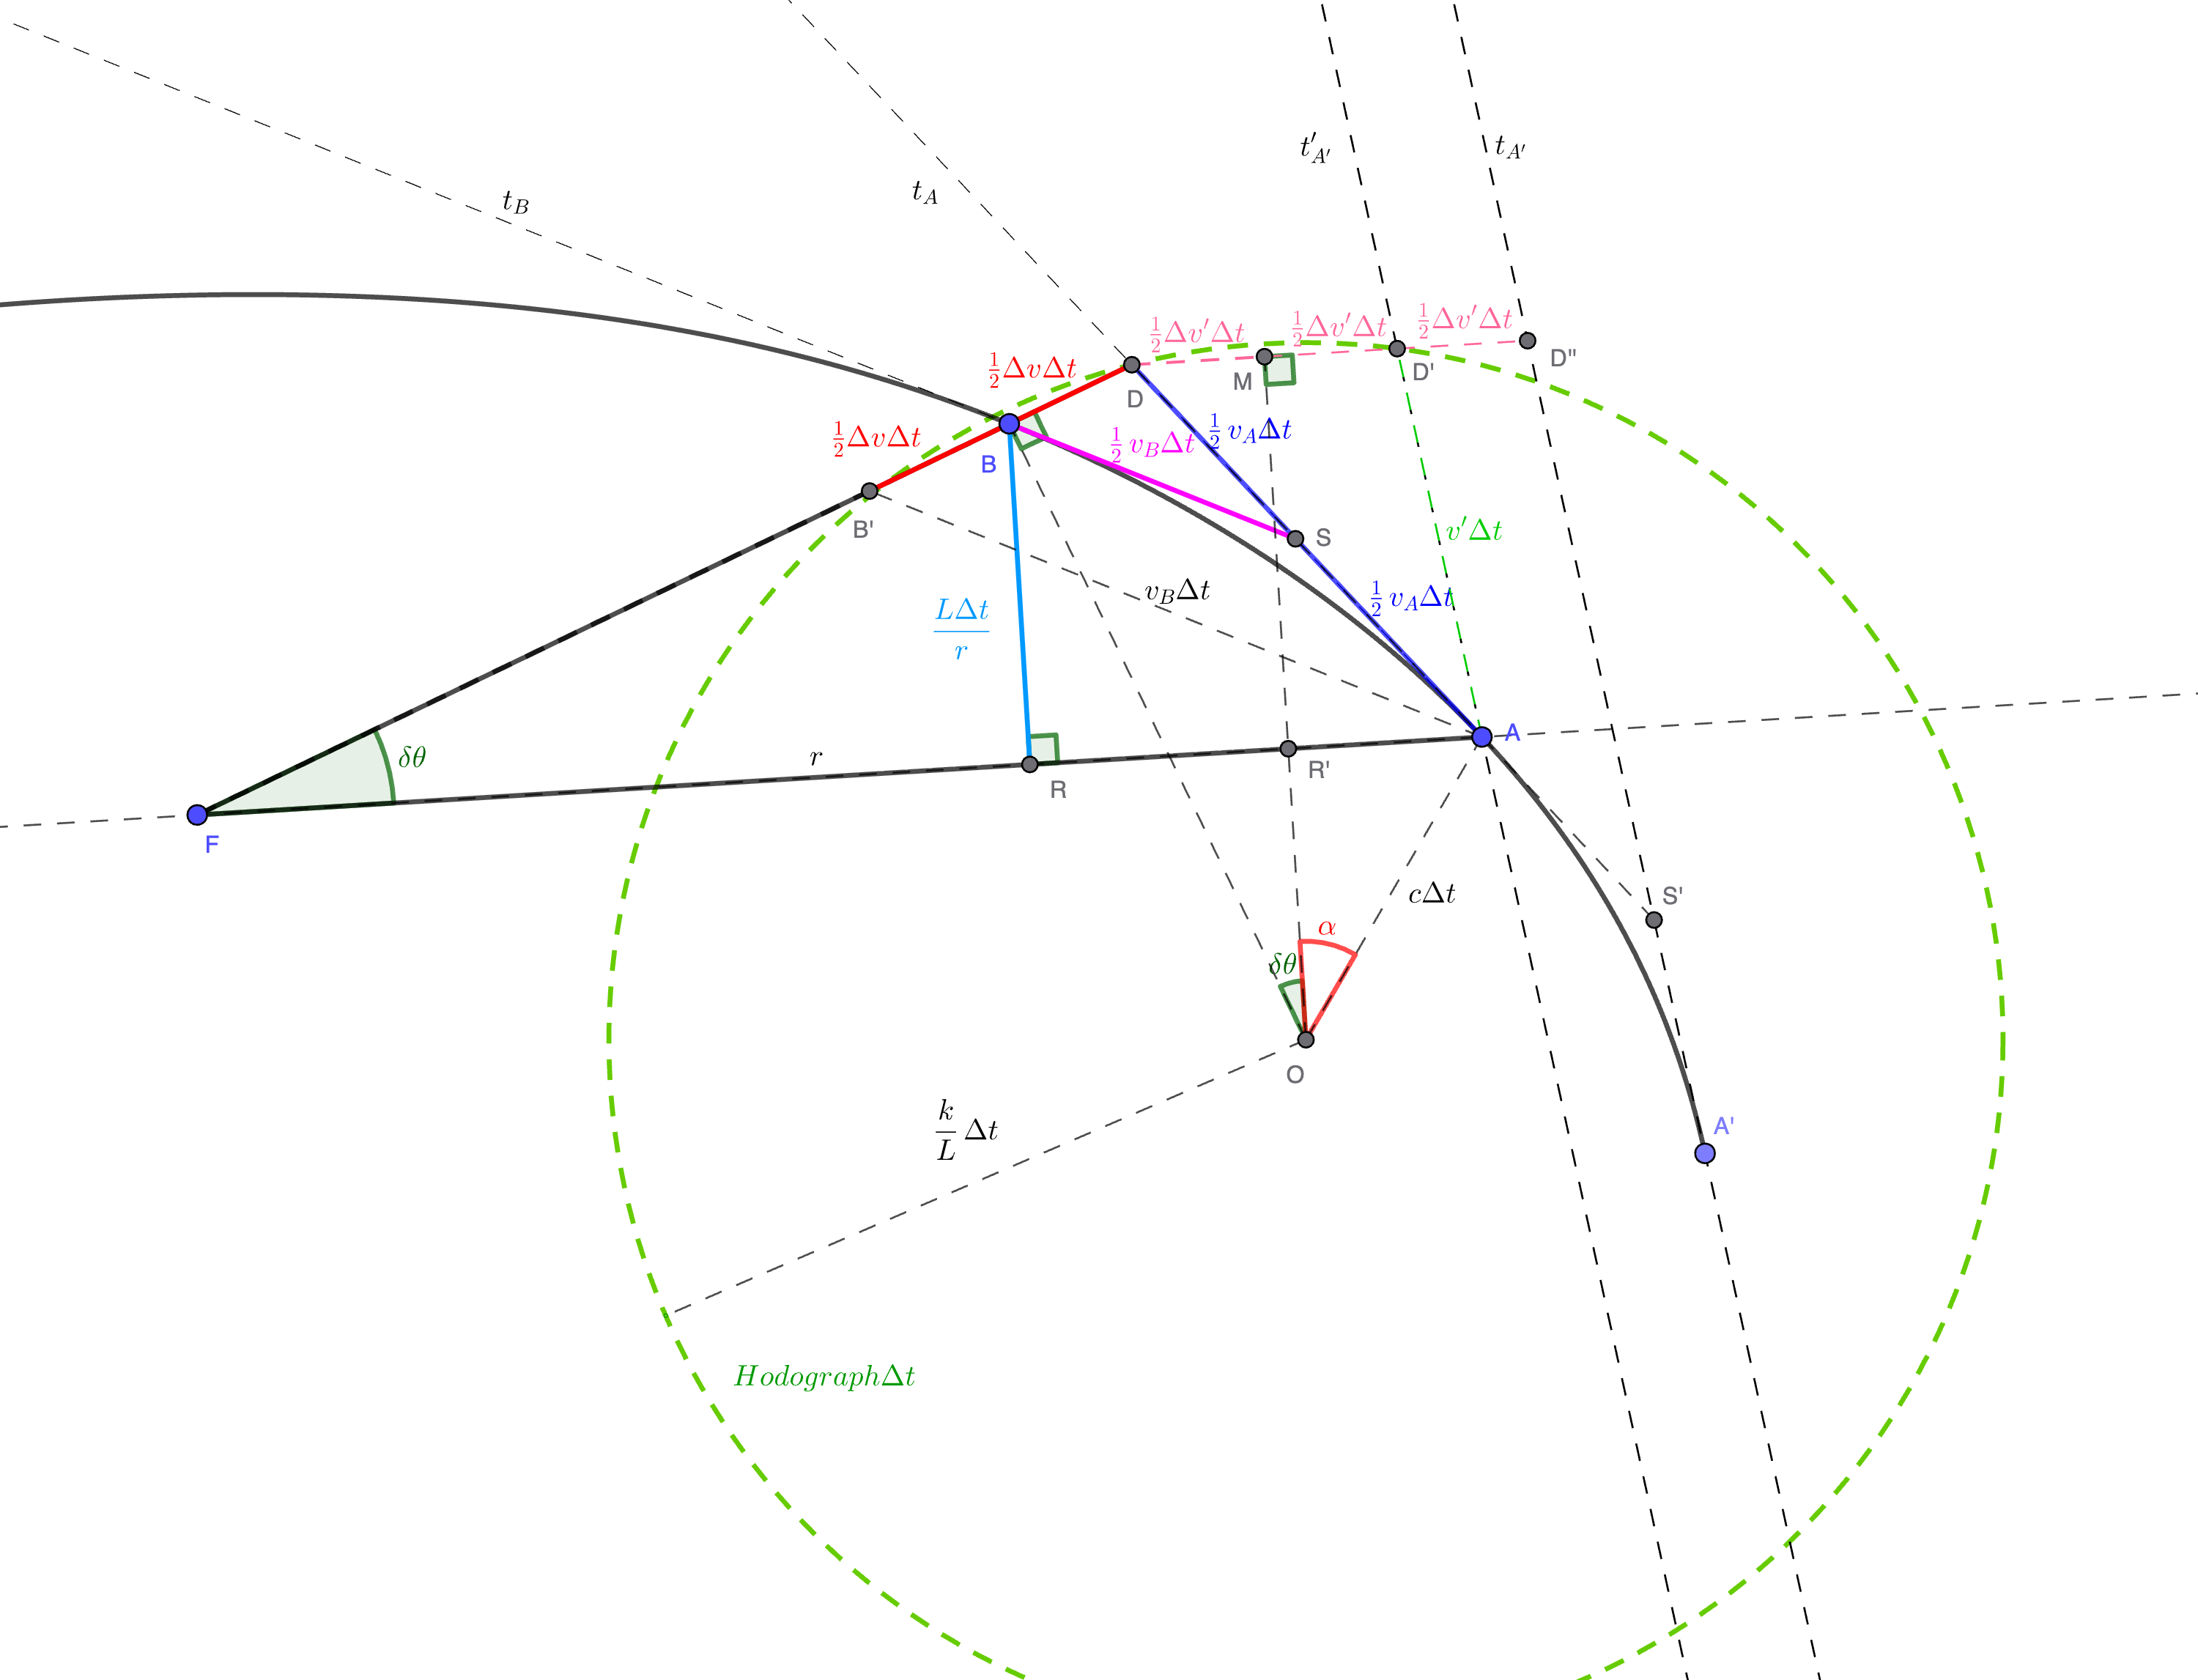
\includegraphics[width=0.95\linewidth]{assets/images/forward_problem.png}
  \caption{Forward-problem construction: previous/current/next velocities ($V_{A'},V_A,V_B$), each scaled by $\Delta t$, are shown on the translated $\Delta t$-scaled hodograph circle, with decomposition $OM=BR+OR'$. As $\Delta t\to 0$, the hodograph circle and all lengths proportional to $\Delta t$ shrink accordingly, while the deflection segments proportional to $\Delta v\,\Delta t$ shrink faster, all to an infinitisimally small circle near point A; the construction is therefore the limit of discrete approximations.}
  \label{fig:forward-problem}
\end{figure}

\begin{proposition}[Hodograph-radius analysis $\Rightarrow$ conic form]
\label[proposition]{prop:inverse-hodograph-proof}
With the notation of \Cref{fig:forward-problem}, the hodograph of $\mathbf v$ is a circle of radius $u$ (hence the $\Delta t$-scaled hodograph circle has radius $u\Delta t$). If the fixed shift is written directly in eccentricity form as
\begin{equation}
  OR'=e\,u\,\Delta t\cos\alpha,
\end{equation}
then
\begin{equation}
  \frac1r=\frac{\mu}{L^2}\left(1-e\cos\alpha\right)
  \quad\Longleftrightarrow\quad
  r(\alpha)=\frac{p}{1-e\cos\alpha},
  \qquad
  p=\frac{L^2}{\mu},
\label{eq:proof1f-r-alpha}
\end{equation}
For a direct geometric interpretation of this polar form in the ellipse construction, see the discussion following \Cref{subsec:ellipse-proof2f}, especially \Cref{eq:ellipse-vn-polar-geom}.
Moreover,
\begin{equation}
  \begin{aligned}
    e<1,\;=1,\;>1
    &\Longleftrightarrow
    \text{velocity-origin inside/on/outside hodograph circle}\\
    &\Longleftrightarrow
    \text{ellipse/parabola/hyperbola}.
  \end{aligned}
\label{eq:proof1f-regimes}
\end{equation}
\end{proposition}

\begin{proof}
In \Cref{fig:forward-problem}, the previous, current, and next velocities ($V_{A'},V_A,V_B$) are placed together in velocity space after scaling by $\Delta t$; this is exactly the translated $\Delta t$-scaled hodograph circle used in the relations below.

First, $\Delta v$ depends only on $\Delta\theta$.
Over a short interval $\Delta t$,
\begin{equation}
  \Delta v=a\,\Delta t=\frac{\mu}{r^2}\Delta t.
\end{equation}
From $L=r^2\dot\theta$, one has $\Delta t=\frac{r^2}{L}\Delta\theta$. Hence
\begin{equation}
  \Delta v=\frac{\mu}{r^2}\cdot\frac{r^2}{L}\Delta\theta=\frac{\mu}{L}\Delta\theta=u\,\Delta\theta,
  \qquad
  \frac{\Delta v}{\Delta\theta}=u\ \text{(constant)}.
\label{eq:inverse-step1}
\end{equation}

Next, conclude the hodograph-circle radius.
Because the force is central, $\Delta\mathbf v$ is radial inward. As $FA$ turns by $\Delta\theta$, the direction of $\Delta\mathbf v$ turns by the same $\Delta\theta$, while its magnitude is $u\,\Delta\theta$ by \eqref{eq:inverse-step1}. Thus the velocity-tip polygon is the equal-angle, equal-arc-length limit of an inscribed circle polygon, so the hodograph is a circle of radius $u$. Multiplying by $\Delta t$ gives
\begin{equation}
  OM=u\,\Delta t.
\label{eq:inverse-step2}
\end{equation}

Then, use tangential displacement.
The tangential speed is $v_\theta=L/r$, hence
\begin{equation}
  BR=v_\theta\Delta t=\frac{L}{r}\Delta t.
\label{eq:inverse-step3}
\end{equation}

Now use the key geometry in the plot.
From the translated-circle construction, $OM=MR'+OR'$ and $MR'=BR$, so
\begin{equation}
  OM=BR+OR'.
\label{eq:inverse-step4}
\end{equation}
Assume
\begin{equation}
  OR'=e\,u\,\Delta t\cos\alpha.
\label{eq:inverse-step5}
\end{equation}
Substitute \eqref{eq:inverse-step2}, \eqref{eq:inverse-step3}, \eqref{eq:inverse-step5} into \eqref{eq:inverse-step4}:
\begin{equation}
  u\Delta t=\frac{L}{r}\Delta t+e\,u\,\Delta t\cos\alpha.
\end{equation}
Cancel $\Delta t$:
\begin{equation}
  u=\frac{L}{r}+e\,u\cos\alpha
  \quad\Longrightarrow\quad
  \frac1r=\frac{u}{L}\left(1-e\cos\alpha\right)
  =\frac{\mu}{L^2}\left(1-e\cos\alpha\right).
\end{equation}
This is equivalent to
\begin{equation}
  r(\alpha)=\frac{p}{1-e\cos\alpha},
  \qquad
  p=\frac{L^2}{\mu},
\end{equation}

Finally, classify by the origin position in velocity space.
The hodograph circle has radius $u$, and the velocity-origin offset has magnitude $eu$. Hence the origin is inside/on/outside the hodograph circle according as $eu<u$, $eu=u$, $eu>u$, i.e. $e<1,=1,>1$. These are precisely the ellipse/parabola/hyperbola regimes.
\end{proof}
This concludes the first forward-problem proof, which is a direct infinitesimal version of the hodograph construction. In the next section, the second proof follows a geometric insight similar to Feynman's Lost Lecture method, with stronger emphasis on the auxiliary circle as a proxy for the hodograph.
